\section{RAILS analyse} \label{app:railsAnalysis}
Het eerste prototype die werkt staat. Nu is het handig om te kijken wat er verbeterd kan worden aan het ontwerp.
Hiervoor gaat de RAILS analyse gebruikt worden. RAILS staat voor Revision, Algoritmes, Interaction, Lookuptables, Sleep. Deze zullen 
alle 5 hieronder besproken worden. 

\subsection{Revision}
Qua hardware is er alleen identificeren van je eigen ID. Doormiddel van een port laag maken kan er gekeken worden welk ID er aan de node 
gemaakt gaat worden. De rest van het protoype is modulair in software gemaakt. In onderstaande afbeelding \ref{fig:AbstractionLayer} is de abstartie laag van de 
software te zien. 

\begin{figure}[h]
    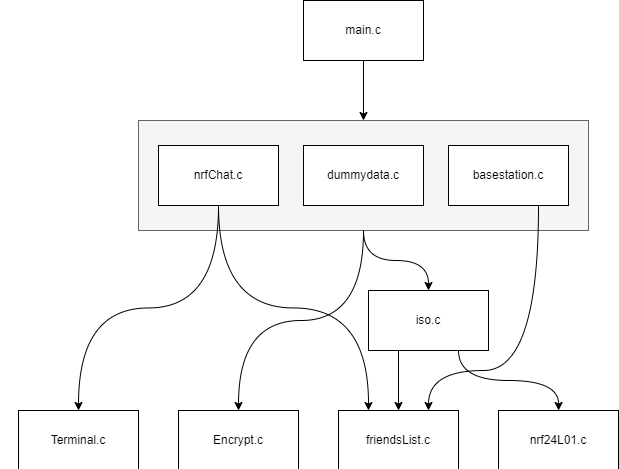
\includegraphics[scale=0.5]{appendices/foto's/AbstractionLayer.drawio.png}
    \caption{Abstractie laag van software}
    \label{fig:AbstractionLayer}
    \end{figure}

\subsection{Algoritmes}
Het enige qua algoritme dat beter kan is de encryptie. Er is nu voor een simpel en snel bedacht algortime gekozen. Deze is als basis goed,
maar als er een netwerk is waarbij data echt strikt geheim is dan moet er wel gekeken worden naar een beter algoritme. Het kost nu niet 
zo veel tijd om het huidige algortime te kraken.

\subsection{Interaction}
Het enige waar tijdens het werk niet fijn was waren de limitaties van de door school geleverde spullen. Deze zorgen ervoor dat de 
efficientie laag is en het energieverbruik hoog ligt. Er zou beter onderzoek moeten komen naar welke hardware beter is om te gebruiken.
Tijdens het process is het ook voorgekomen dat iets brak en de kosten van repareren was hoger omdat het een ouder model was. Er zouden oplossingen
moeten zijn zoals een beschermingshoes bij een erg fragiel onderdeel of een goedwerkend, efficientere, nieuwer scherm. Die uiteindelijk ook 
qua kosten minder zou zijn.

\subsection{Lookuptables}


\subsection{Sleep}
De software gebruikt nu ook alleen maar de hardware onderdelen die nodig zijn. Misschien is het handig, maar dit moet onderzocht worden, 
om eenmalig een unieke ID te maken met de hardware en dat daarna deze pins worden afgesloten. Hier komt het punt die bij Interactie ook is 
besproken. De Xmega chip is erg gelimiteerd met de kloksnelheid. Hier zal meer onderzoek voor gedaan worden, maar de chip kan er ook voor zorgen 
dat het netwerk efficienter zal gaan lopen. Door bijvoorbeeld een chip te kiezen die laag is in energie verbruik, maar ook alleen de functies heeft die 
het netwerk nodig heeft. Dan kan er een chip uitgekozen worden die alleen de functionele blokken bevat die nu gebruikt worden.